\documentclass{beamer}
\usetheme[titlepagelogo=../img/logo-unicam,% Logo for the first page
		  language=english,
		  bullet=triangle,
		  color=green,
          secondsupervisor=true,
          secondlogo=true,
          assistantsupervisor=true,
         ]{TorinoTh}
\usepackage[beamer,customcolors]{hf-tikz}
\usepackage{glossaries}
\usepackage{tikz}
\usepackage{hyperref}
\usepackage[backend=biber,style=numeric,sorting=none]{biblatex}  % Use numbered citations
\usepackage{csquotes}
\usetikzlibrary{shapes.geometric, arrows, positioning, fit}

\hfsetfillcolor{alerted text.fg!10}
\hfsetbordercolor{alerted text.fg}

\author{Piermichele Rosati}
\rel{Prof. Emanuele Laurenzi}
\assistantsupervisor{Prof. Michela Quadrini}
\title{\small \textit{A Hybrid AI Approach for Recommending Collaborators in Research Projects}}
\ateneo{\scriptsize University of Camerino \\\&\\ University of Applied Sciences and Arts Northwestern Switzerland}
\date{\textit{MSc in Computer Science and Business Information Systems}\\\today}
\titlepagesecondlogo{../img/logo-fhnw}

%%% to remove square brackets from citations %%%
\makeatletter
\def\@biblabel#1{}
\renewcommand\@cite[2]{{#1\if@tempswa,\nolinebreak[3] #2\fi}}
\makeatother
%%%%%%

% Ensure no color formatting is applied to glossary terms
\renewcommand*{\glstextformat}[1]{\textcolor{black}{#1}}

\glsdisablehyper

\renewcommand*{\bibfont}{\tiny}
\addbibresource{bibliography.bib}

% Fix citation color to black
\usepackage{hyperref}
\hypersetup{
    colorlinks=true, 
    urlcolor=black, 
    linkcolor=black, 
    citecolor=black  % Ensures citations are black
}

\begin{document}

\addtobeamertemplate{frametitle}{}{%
\begin{tikzpicture}[remember picture,overlay]
\node[anchor=west,yshift=-20pt] at (current page.north west) {
\includegraphics[height=1.1cm]{../img/logo-unicam-notext.png}};
\node[anchor=north east,yshift=-5pt] at (current page.north east) {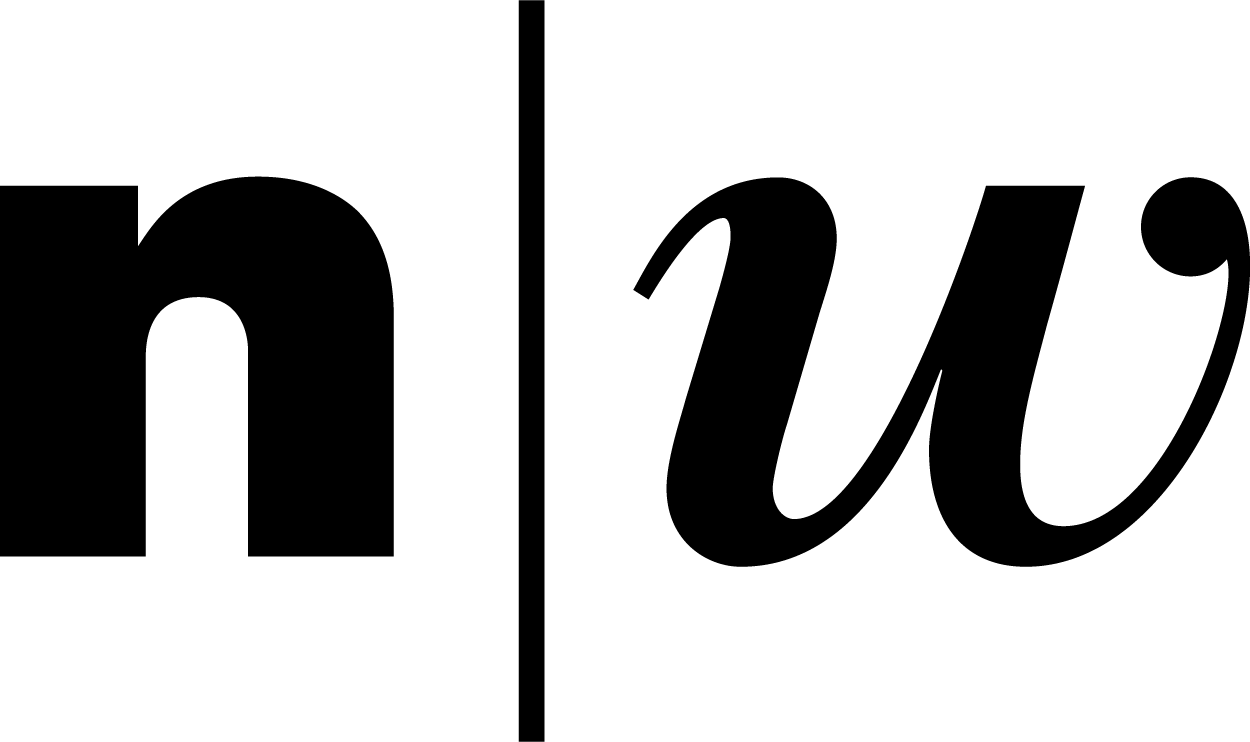
\includegraphics[height=0.9cm]{../img/logo-fhnw-notext.png}};
\end{tikzpicture}
\vspace{-0.5cm}
}

\titlepageframe

\setbeamertemplate{section in toc}[sections numbered]
\setbeamertemplate{subsection in toc}[subsections numbered]
\setbeamercolor{section in toc}{fg=forestgreen}
%\setbeamercolor{subsection in toc}{fg=red}
\definecolor{black}{rgb}{0,0,0}
\setbeamercolor{bibliography entry author}{fg=black}
\setbeamercolor{bibliography entry title}{fg=black}
\setbeamercolor{bibliography entry journal}{fg=black}
\setbeamercolor{bibliography item}{fg=black}
\setbeamercolor{cite}{fg=black}

\newacronym{srq}{SRQ}{Sub-Research Question}
\newacronym{kg}{KG}{Knowledge Graph}
\newacronym{ai}{AI}{Artifical Intelligence}
\newacronym{llm}{LLM}{Large Language Model}
\newacronym{dnn}{DNN}{Deep Neural Network}
\newacronym{rag}{RAG}{Retrieval Augmented Generation}
\newacronym{cbf}{CBF}{Content-Based Filtering}
\newacronym{cf}{CF}{Collaborative Filtering}
\newacronym{recsys}{RecSys}{Recommender System}
\newacronym{cordis}{CORDIS}{Community Research and Development Information Service}
\newacronym{fp7}{FP7}{Seventh Framework Programme}
\newacronym{h2020}{H2020}{Horizon 2020}
\newacronym{eurio}{EURIO}{EUropean Research Information Ontology}
\newacronym{dsr}{DSR}{Design Science Research}
\newacronym{ar}{AR}{Answer Relevancy}
\newacronym{cp}{CP}{Context Precision}
\newacronym{cr}{CR}{Context Recall}
\newacronym{cer}{CER}{Context Entity Recall}
\newacronym{ss}{SS}{Answer Semantic Similarity}
\newacronym{ac}{AC}{Answer Correctness}
\newacronym{ragas}{RAGAs}{Retrieval-Augmented Generation Assessment}
\newacronym{rdf}{RDF}{Resource Description Framework}

%%% showing outline before each section %%%
% \AtBeginSection[]
% {
% \begin{frame}<beamer>
% \frametitle{Outline}
% \tableofcontents[currentsection]
% \end{frame}
% }

%%% showing outline only at the beginning %%%
%\begin{tframe}{Outline}
%    \tableofcontents
%\end{tframe}

\section{Introduction}
\begin{tframe}{Consortia}
%Research collaboration is the process where researchers from various fields, institutions, or disciplines work together to achieve shared scientific objectives \cite{KATZ19971}.

%\vspace{0.2cm}

A \textbf{consortium} is a group of organizations or individuals that collaborate to achieve a common objective \cite{KATZ19971}.

\vspace{0.5cm}

Successful research proposals require a \textbf{consortium} experienced in the topics of the call.

\vspace{0.5cm}

\textbf{Consortia advantages}:
\begin{adv}
    \item Shared resources and infrastructure
    \item Access to complementary expertise
    \item Cost sharing and risk reduction
    \item Improved innovation and research outcomes
\end{adv}

\end{tframe}
%
%\section{Literature Review}
%\begin{tframe}{Literature of Knowledge Graphs}
    A \gls{kg} refers to a semantic network graph which is consisted of diverse entities, concepts, and relationships in the real world. %(\cite{Hogan2021});
    %It is used to formally describe various things and their associations in the real world.
    \vspace{0.2cm}

    \textbf{Applications}: Social networks, IoT, Healthcare, Search Engines\ldots
    \vspace{0.2cm}

    \begin{minipage}[t]{.5\linewidth}
        \textbf{Benefits of \glspl{kg}:}
        \begin{adv}
            \item Data unification
            \item Easy availability
            \item Semantic meaning
            \item Easier integration
            \item Discovery of hidden patterns
            \item Faster decision making
        \end{adv}
    \end{minipage}%
    \hfill%
    \begin{minipage}[t]{.5\linewidth}
        \textbf{Challenges of \glspl{kg}:}
        \begin{disadv}
            \item Knowledge graph embeddings
            \item Knowledge acquisition
            \item Knowledge completion
            \item Knowledge fusion
            \item Knowledge reasoning
        \end{disadv}
    \end{minipage}
\end{tframe}
%
\begin{tframe}{Literature of Graph Neural Networks}
    GNNs are deep learning based methods that operate on graph domain.
    \vspace{0.2cm}

    \textbf{Applications}: Recommender systems, BioInformatics, Computer Vision\ldots
    \vspace{0.2cm}

    \textbf{Tasks:} Node-Level, Edge-Level, Graph-Level.
    \vspace{0.2cm}

    \begin{minipage}[t]{.5\linewidth}
        \textbf{Benefits of GNNs:}
        \begin{adv}
            \item Modeling relational data;
            \item Generalization to\\ arbitrary graphs;
            \item Capturing complex\\ relationships;
            \item Representation learning.
        \end{adv}
    \end{minipage}%
    \hfill%
    \begin{minipage}[t]{.5\linewidth}
        \textbf{Challenges of GNNs:}
        \begin{disadv}
            \item Scalability;
            \item Data quality and noise;
            \item Model interpretability;
            \item Over-smoothing;
            \item Graph isomorphism problem.
        \end{disadv}
    \end{minipage}
\end{tframe}
%
% \begin{tframe}{Application of KGs}
%     \begin{figure}[htbp]
%         \centering
%      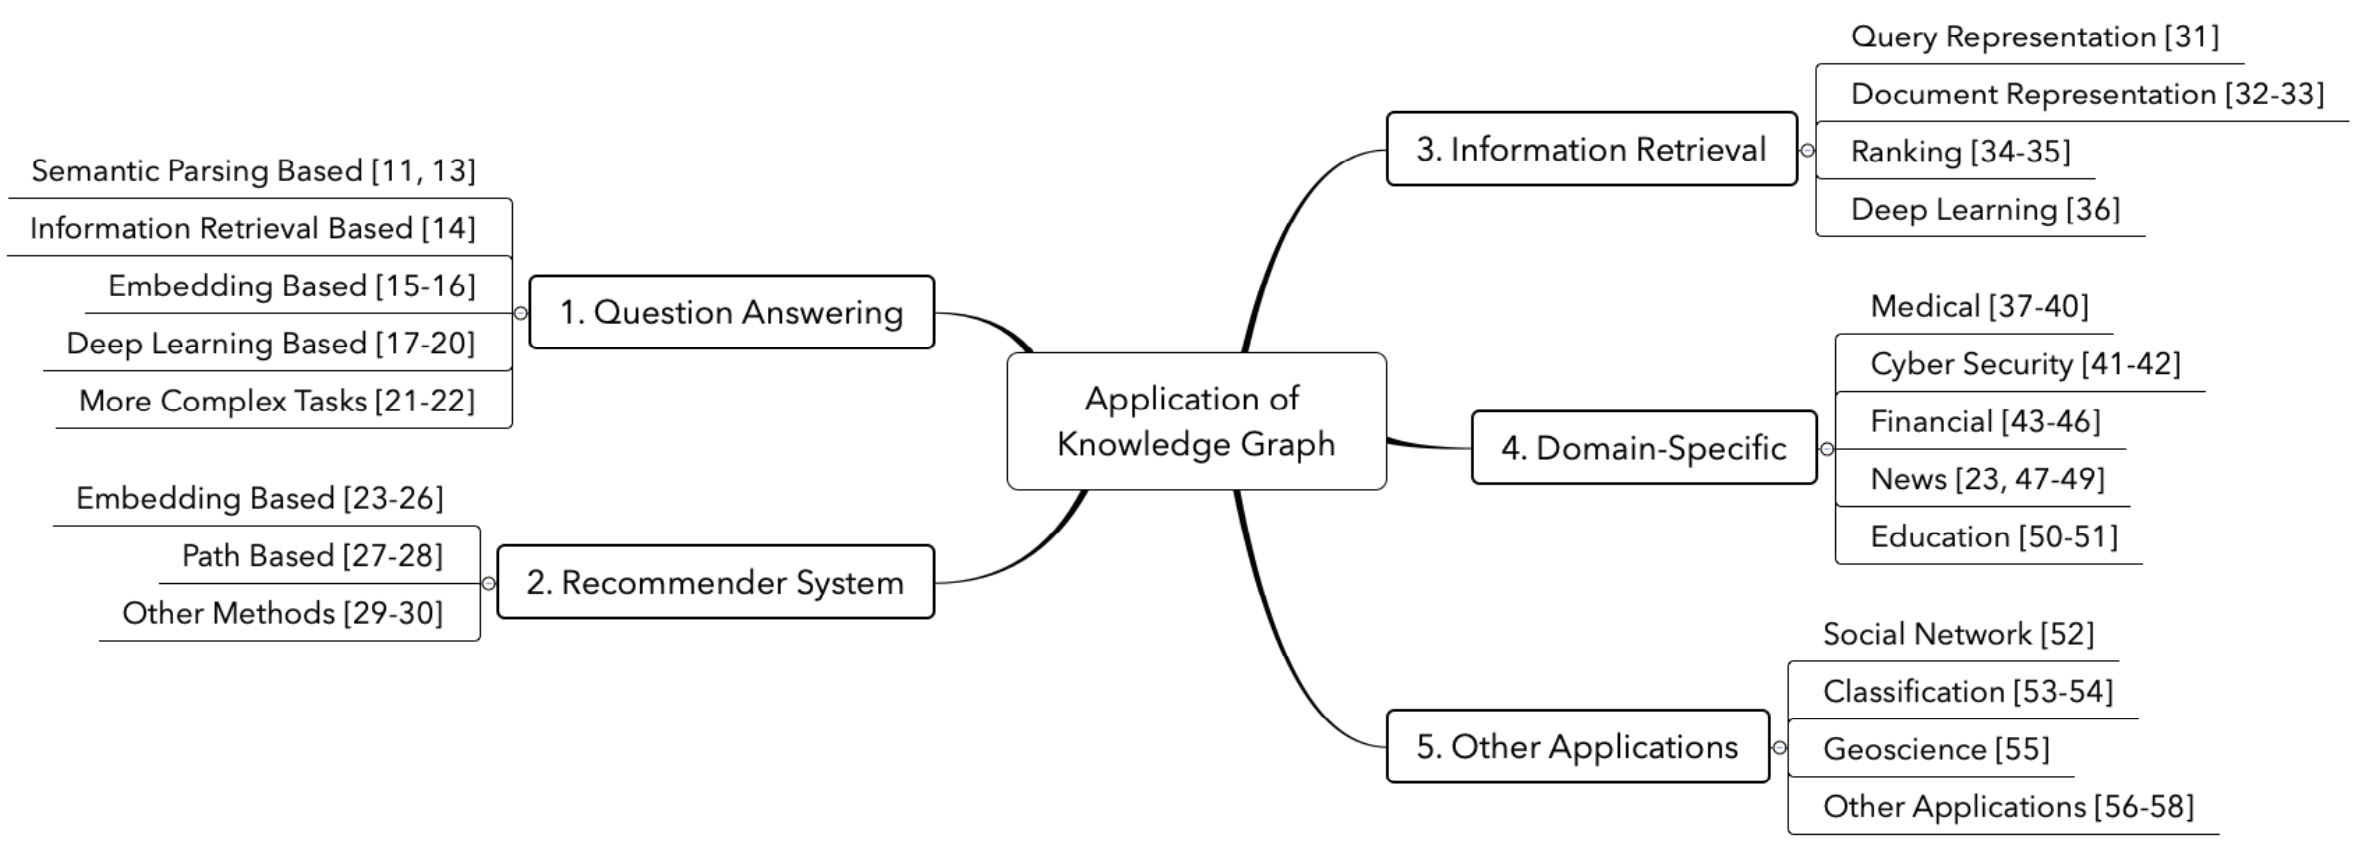
\includegraphics[width=0.9\textwidth]{../img/literature-review/application-field-kg.png}
%      \caption{Application fields of KGs (\cite{Zou2020})}
%     \end{figure}
% \end{tframe}
% \begin{tframe}{Literature of Graph Neural Networks}
% Graph Neural Networks (GNNs) are deep learning based methods that operate on graph domain (non-Euclidean space) (\cite{Wu2021}).
% \newline
% \\ GNNs were introduced when Convolutional Neural Networks (CNNs) failed to achieve optimal results due to the arbitrary size of the graph and complex structure. 
% \newline
% \\ GNN aims to map the node features to node embeddings such that 2 embeddings are ''similar`` if the 2 nodes are ''similar`` in the graph.
% \end{tframe}
% %
% \begin{tframe}{GNN Tasks}
%     \begin{itemize}
%         \item \textbf{Node-Level}: node classification, node regression, node clustering, etc;
%         \item \textbf{Edge-Level}: edge classification and link prediction;
%         \item \textbf{Graph-Level}: graph classification, graph regression, and graph matching.
%     \end{itemize}
% \end{tframe}
% %
% \begin{tframe}{How GNN works}
%     \begin{enumerate}
%         \item \textbf{Message Passing}: is the process of taking node features of the neighbours, transforming them, and ''passing`` them to the source node. This process is repeated, in parallel, for all nodes in the graph. In that way, all neighbourhoods are examined by the end of this step.
%         \item \textbf{Aggregation}: is the process to ''combine`` the transformed messages and the source node together;
%         \item \textbf{Update}: using these aggregated messages, the GNN layer now has to update the source node $\mathnormal{i}$'s features. At the end of this update step, the node should not only know about itself but its neighbours as well. This is ensured by taking the node $\mathnormal{i}$'s feature vector and combining it with the aggregated messages.
%     \end{enumerate}
% \end{tframe}
% %
% \begin{tframe}{The Message Passing Neural Network (MPNN)}
% The MPNN is the most general GNN model:
% \begin{align*}
%     x_i' = \psi(x_i,~\sigma_{j \in N(i)}~ \phi(x_{i},e_{ij},x_j))
% \end{align*}
% where:
% \begin{itemize}
%     \item $\phi$ is a differentiable \textbf{message} funtion;
%     \item $\sigma$ is a permutation-invariant aggregation function (sum, average, etc.)
%     \item $\psi$ is a differentiable \textbf{update} function;
% \end{itemize}
% \end{tframe}
%
\begin{tframe}{Meeting with Domain Experts}
\begin{itemize}
    \item Stakeholders presentation;
    \item BEMS domain details;
    \item Data representation;
    \item Key challenges.
\end{itemize}
\end{tframe}
%
\begin{tframe}{Literature of Knowledge Graph Completion}
\vspace{-.3cm}
Current real-world KGs are usually incomplete and need an inference engine to predict links and complete the missing facts among entities available in the KG.
\newline
\\Knowledge Graph Completion (KGC) is one of the popular technologies for knowledge supplement. 
\vspace{0.1cm}

\begin{itemize}
    \item \textbf{Link Prediction:} aims to predict missing relationships between entities in a graph;
    
    % \begin{minipage}[t]{.5\linewidth}
    %     \textbf{Benefits:}
    %     \begin{adv}
    %         \item Data augmentation;
    %     \end{adv}
    % \end{minipage}%
    % \hfill%
    % \begin{minipage}[t]{.5\linewidth}
    %     \textbf{Challenges:}
    %     \begin{disadv}
    %         \item Scalability, Data sparsity, Bias, ;
    %     \end{disadv}
    % \end{minipage}
    % \vspace{.1cm}
    \item \textbf{Knowledge Graph Embedding (KGE)}: is a representation of a KG element into a continuous vector space;
    % \begin{minipage}[t]{.5\linewidth}
    %     \textbf{Benefits:}
    %     \begin{adv}
    %         \item GNNs models learn\\ powerful embeddings by\\ using topological structures\\ of KGs;
    %     \end{adv}
    % \end{minipage}%
    % \hfill%
    % \begin{minipage}[t]{.5\linewidth}
    %     \textbf{Challenges:}
    %     \begin{disadv}
    %         \item Treat each triple independently;
    %         %\item fail to cover the complex inherently implicit information in the local neighborhood of a triple;
    %         \item Fail to cover the complex inherently implicit information.
    %     \end{disadv}
    % \end{minipage}
    \item \textbf{GNNs} have been recently applied in KGs to learn powerful embeddings by using topological structures in the KGs.
\end{itemize}
\end{tframe}
\section{Related Work}
\begin{tframe}{Related Work}

\begin{itemize}
    \item Traditional \textbf{recommender systems} such as \gls{cbf} and \gls{cf} suggest relevant items based on user preferences and item features \cite{Plexousakis2005, WEI201729, Lu2012}
    \vspace{.1cm}
    %\item These models often lack transparency and fail to support serendipitous or interdisciplinary recommendations \cite{AIinRecSys, Jagadishwari2023, Iana2021}
    \item \textbf{Deep learning-based models} get high accuracy but do not offer explainable results \cite{Zhao2024}
    \vspace{.1cm}
    %\item To overcome these issues, recent works explore combining external knowledge with neural models
    \item \textbf{\glspl{llm}}, especially when enhanced with \textbf{\gls{rag}}, offer explainability and improved contextual understanding \cite{Deldjoo2024}
    \vspace{.1cm}
    \item A promising direction combining \textbf{\glspl{kg}} and \textbf{\glspl{llm}} is explored in \cite{Yang2024, Pan2024}
\end{itemize}
\end{tframe}
%
\section{Problem Statement}
\begin{tframe}{Problem Statement}
The problem faced in this thesis is to extract IoT data from sensors and representing it using own ontologies/KGs.
\vspace{.5cm}
\begin{itemize}
    \item The sensory IoT data produced by BEMSs need significant curation before it can be used meaningfully.
    \item Large buildings could have thousands of sensors, which make data transfer and management challenging; %(\cite{Bae2021});
    \item High engineering work requiring multiple domain experts.
\end{itemize}
\end{tframe}
%
\section{Research Questions}
\begin{frame}{Research Questions}
\textbf{Main Research Question}:
\begin{center}
	\textit{How can a \gls{kg} and \gls{llm}-based approach enhance the process of suggesting collaborators for research projects?}
\end{center}
\vspace{.2cm}
\textbf{\glspl{srq}}:
\small{
\begin{itemize}
	\item \textbf{\gls{srq}1}: \textit{How can research-related data (e.g., projects, people, affiliations) be modeled into a \gls{kg} for research collaborator recommendation?}
    \item \textbf{\gls{srq}2}: \textit{How can a \gls{kg} and \gls{llm}-based system be designed to efficiently retrieve relevant information from large, heterogeneous data sources to support personalized recommendations?}
    \item \textbf{\gls{srq}3}: \textit{How can the system generate human-readable explanations for its research collaborator recommendations using the \gls{kg} and \gls{llm} outputs?}
\end{itemize}
}
\end{frame}
%
%\section{State of the Art}
%\begin{frame}{State of the Art}
    
\end{frame}
\section{Research Design}
\begin{tframe}{Research Methodology}
\framesubtitle{\acrlong{dsr} (\textcite{Hevner2010} adapted from \textcite{Vaishnavi2007})}
    \begin{figure}[htbp]
        \centering
        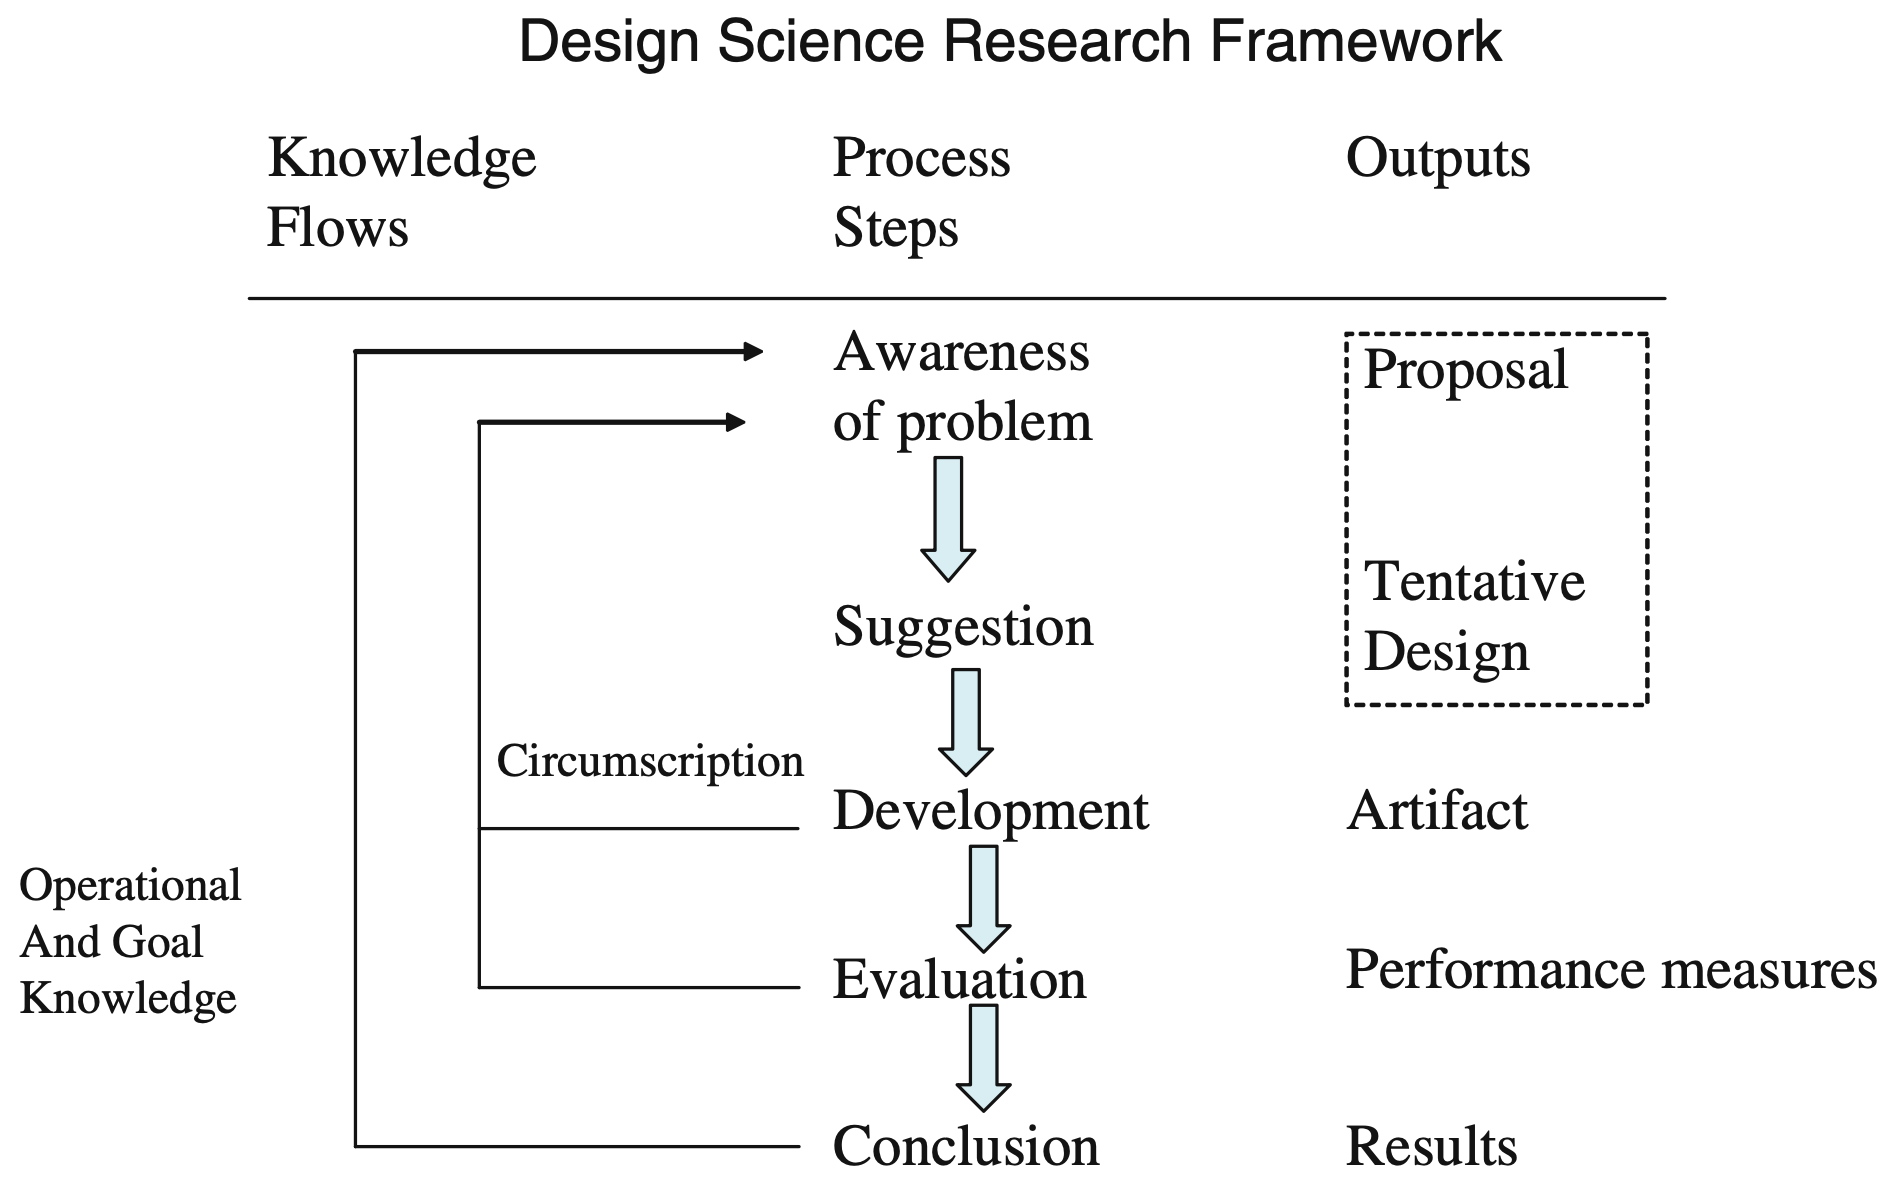
\includegraphics[width=.8\textwidth]{../img/research-design/design-science-research-framework.png}
    \end{figure}
\end{tframe}
%
\section{Dataset}
\begin{tframe}{Dataset}
\begin{columns}
    \begin{column}{0.53\textwidth}
        %\vspace{-2cm}

        \textbf{\gls{cordis}}: the EU Commission's main public source for EU-funded research projects \cite{CORDIS_RefData_2018}.
        
        %\vspace{0.5cm}

        %\begin{itemize}
        %    \item the \textbf{\gls{fp7}} for Research and Technological Development (2007-2013)
        %    \item the \textbf{\gls{h2020}} Programme for Research and Innovation (2014-2020)
        %\end{itemize}
        \begin{figure}[htbp]
            \centering
            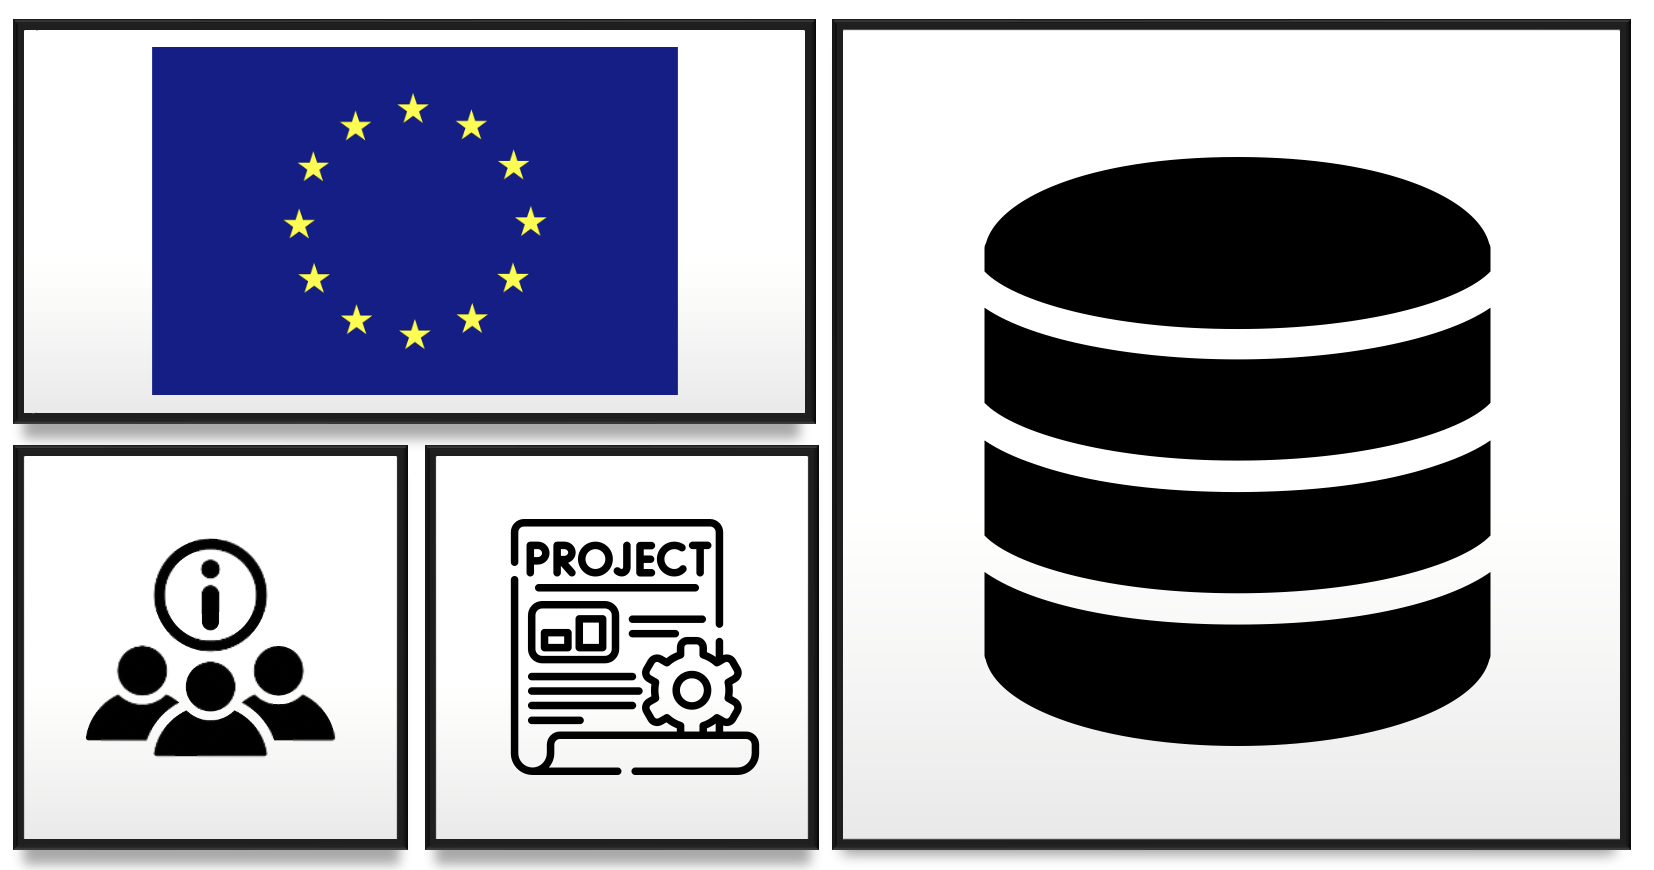
\includegraphics[width=.6\textwidth]{../img/scenario-analysis/cordis.png}
        \end{figure}

        The dataset includes projects information and details from the \textbf{\acrshort{fp7}} \cite{CORDIS_FP7_2015} and \textbf{\acrshort{h2020}} \cite{CORDIS_H2020_2015} programmes.
    \end{column}
    \begin{column}{0.4\textwidth}
        \vspace{-.5cm}
        \begin{figure}[htbp]
            \centering
            
\includegraphics[width=.8\textwidth]{../img/scenario-analysis/example-project.png}
        \end{figure}
    \end{column}
\end{columns}
\end{tframe}
%
\section{Artifact Design}
\begin{tframe}{Ontology Selection}
The \gls{eurio}: data model that formalizes and makes available structured, machine-readable data on EU-funded research projects.

\begin{columns}
    \begin{column}{0.48\textwidth}
      \vspace{-.5cm}
        \begin{itemize}
            \item Semantic model of research information, e.g., projects, calls, funding schemes, organizations, people \ldots
            \vspace{.2cm}
            \item \textbf{\gls{eurio} \gls{kg}} \cite{CORDIS_EURIO_2022}: an \acrshort{rdf} \gls{kg} built from \gls{cordis} data
        \end{itemize}
    \end{column}
    \begin{column}{0.48\textwidth}
      \begin{figure}
        \centering
        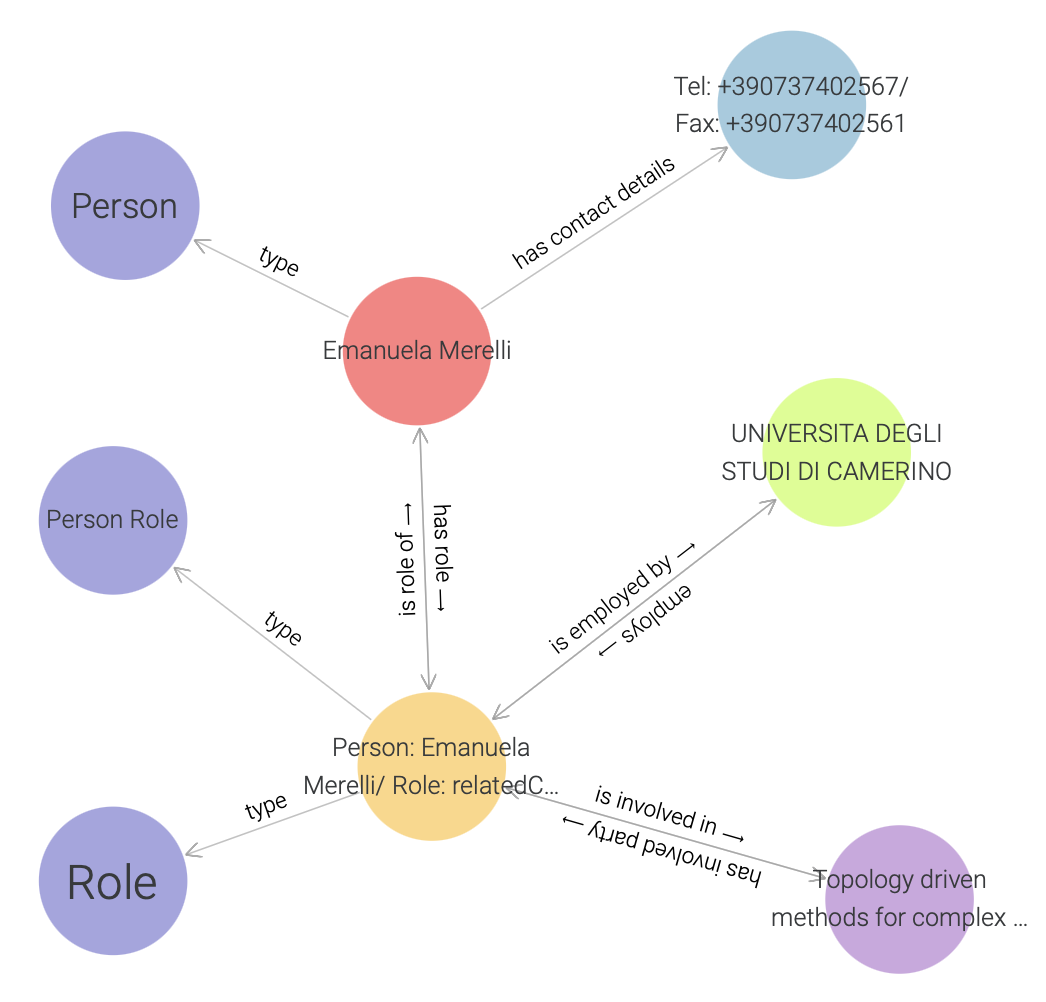
\includegraphics[width=.95\linewidth]{../img/architecture/example-merelli.png}
      \end{figure}
    \end{column}
  \end{columns}

\end{tframe}
%
\begin{tframe}{Recommendation Types}
The recommendation strategy leverages structured data properties and relationships in the \gls{eurio} \gls{kg} to generate context-aware suggestions.

\vspace{0.5cm}

\begin{columns}
    \begin{column}{0.48\textwidth}
      \begin{figure}
        \centering
        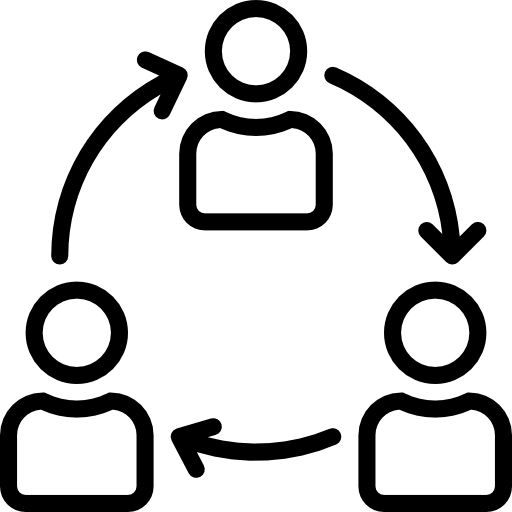
\includegraphics[width=.4\linewidth]{../img/architecture/strategy-collaborators.png}
      \end{figure}
      \centering
      \textbf{Research collaborators recommendation}
    \end{column}
    \begin{column}{0.48\textwidth}
      \begin{figure}
        \centering
        
\includegraphics[width=.4\linewidth]{../img/architecture/strategy-consortium.png}
      \end{figure}
      \centering
      \textbf{Consortium organisations recommendation}
    \end{column}
  \end{columns}
\end{tframe}
%
\begin{frame}{GraphRAG Architecture}
\framesubtitle{(from \textcite{Singh2025})}
    \begin{figure}
        \centering
        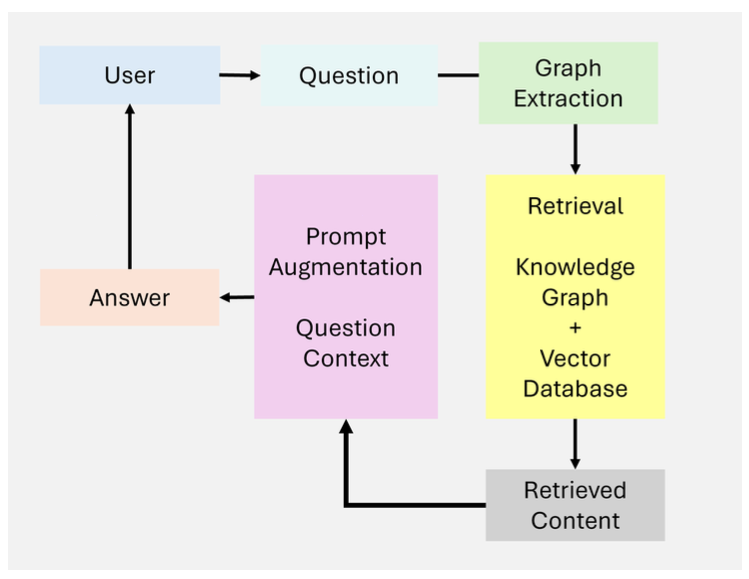
\includegraphics[width=.7\textwidth]{../img/architecture/graphRAG.png}
    \end{figure}
    \centering
\end{frame}
%
\begin{frame}{AgenticRAG Architecture}
\framesubtitle{(from \textcite{Singh2025})}
    \begin{figure}
        \centering
        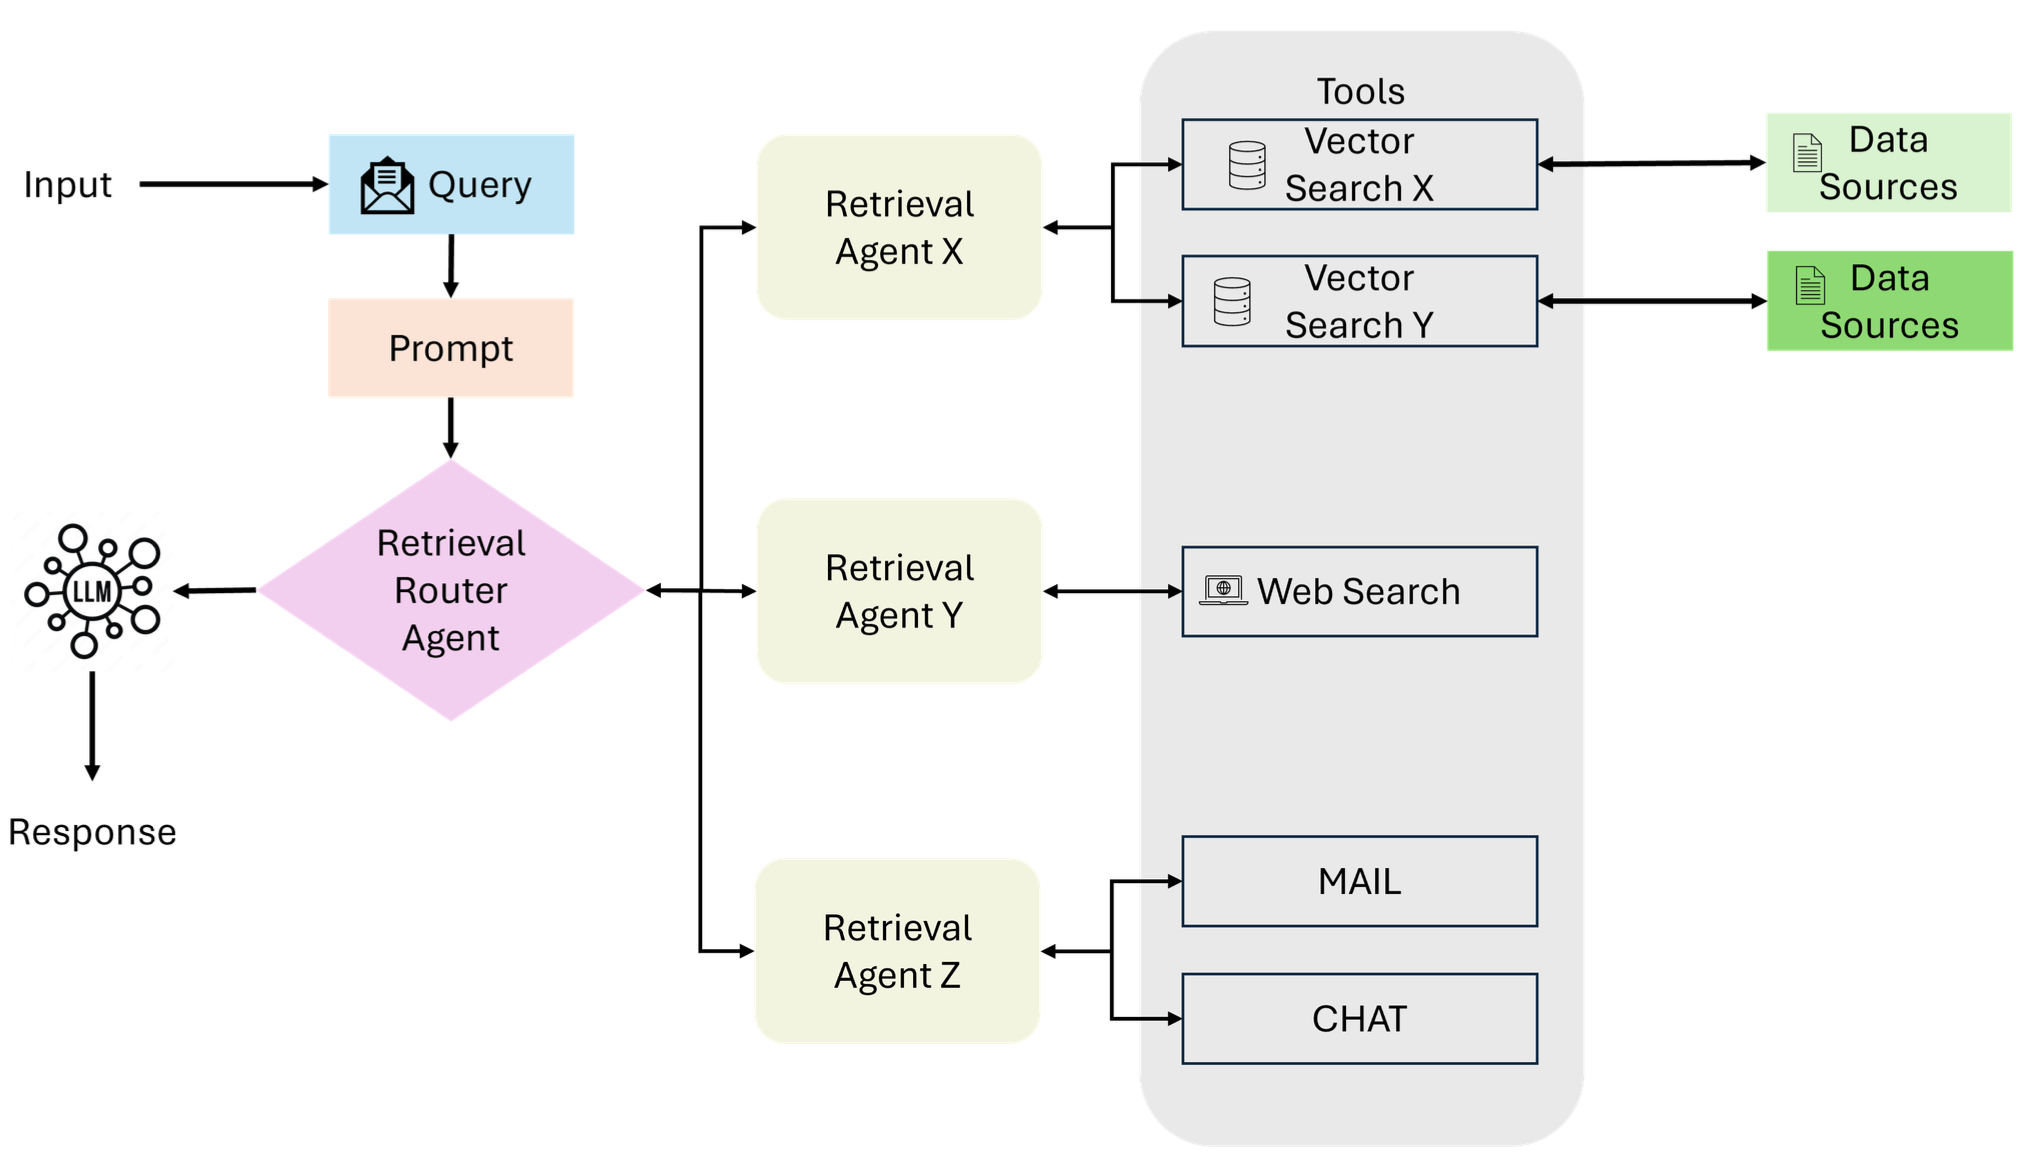
\includegraphics[width=.9\textwidth]{../img/architecture/multi-agent-agentic-rag.png}
    \end{figure}
    \centering
\end{frame}
%
\begin{frame}{Artifact Design}
    
    \begin{figure}
        \centering
        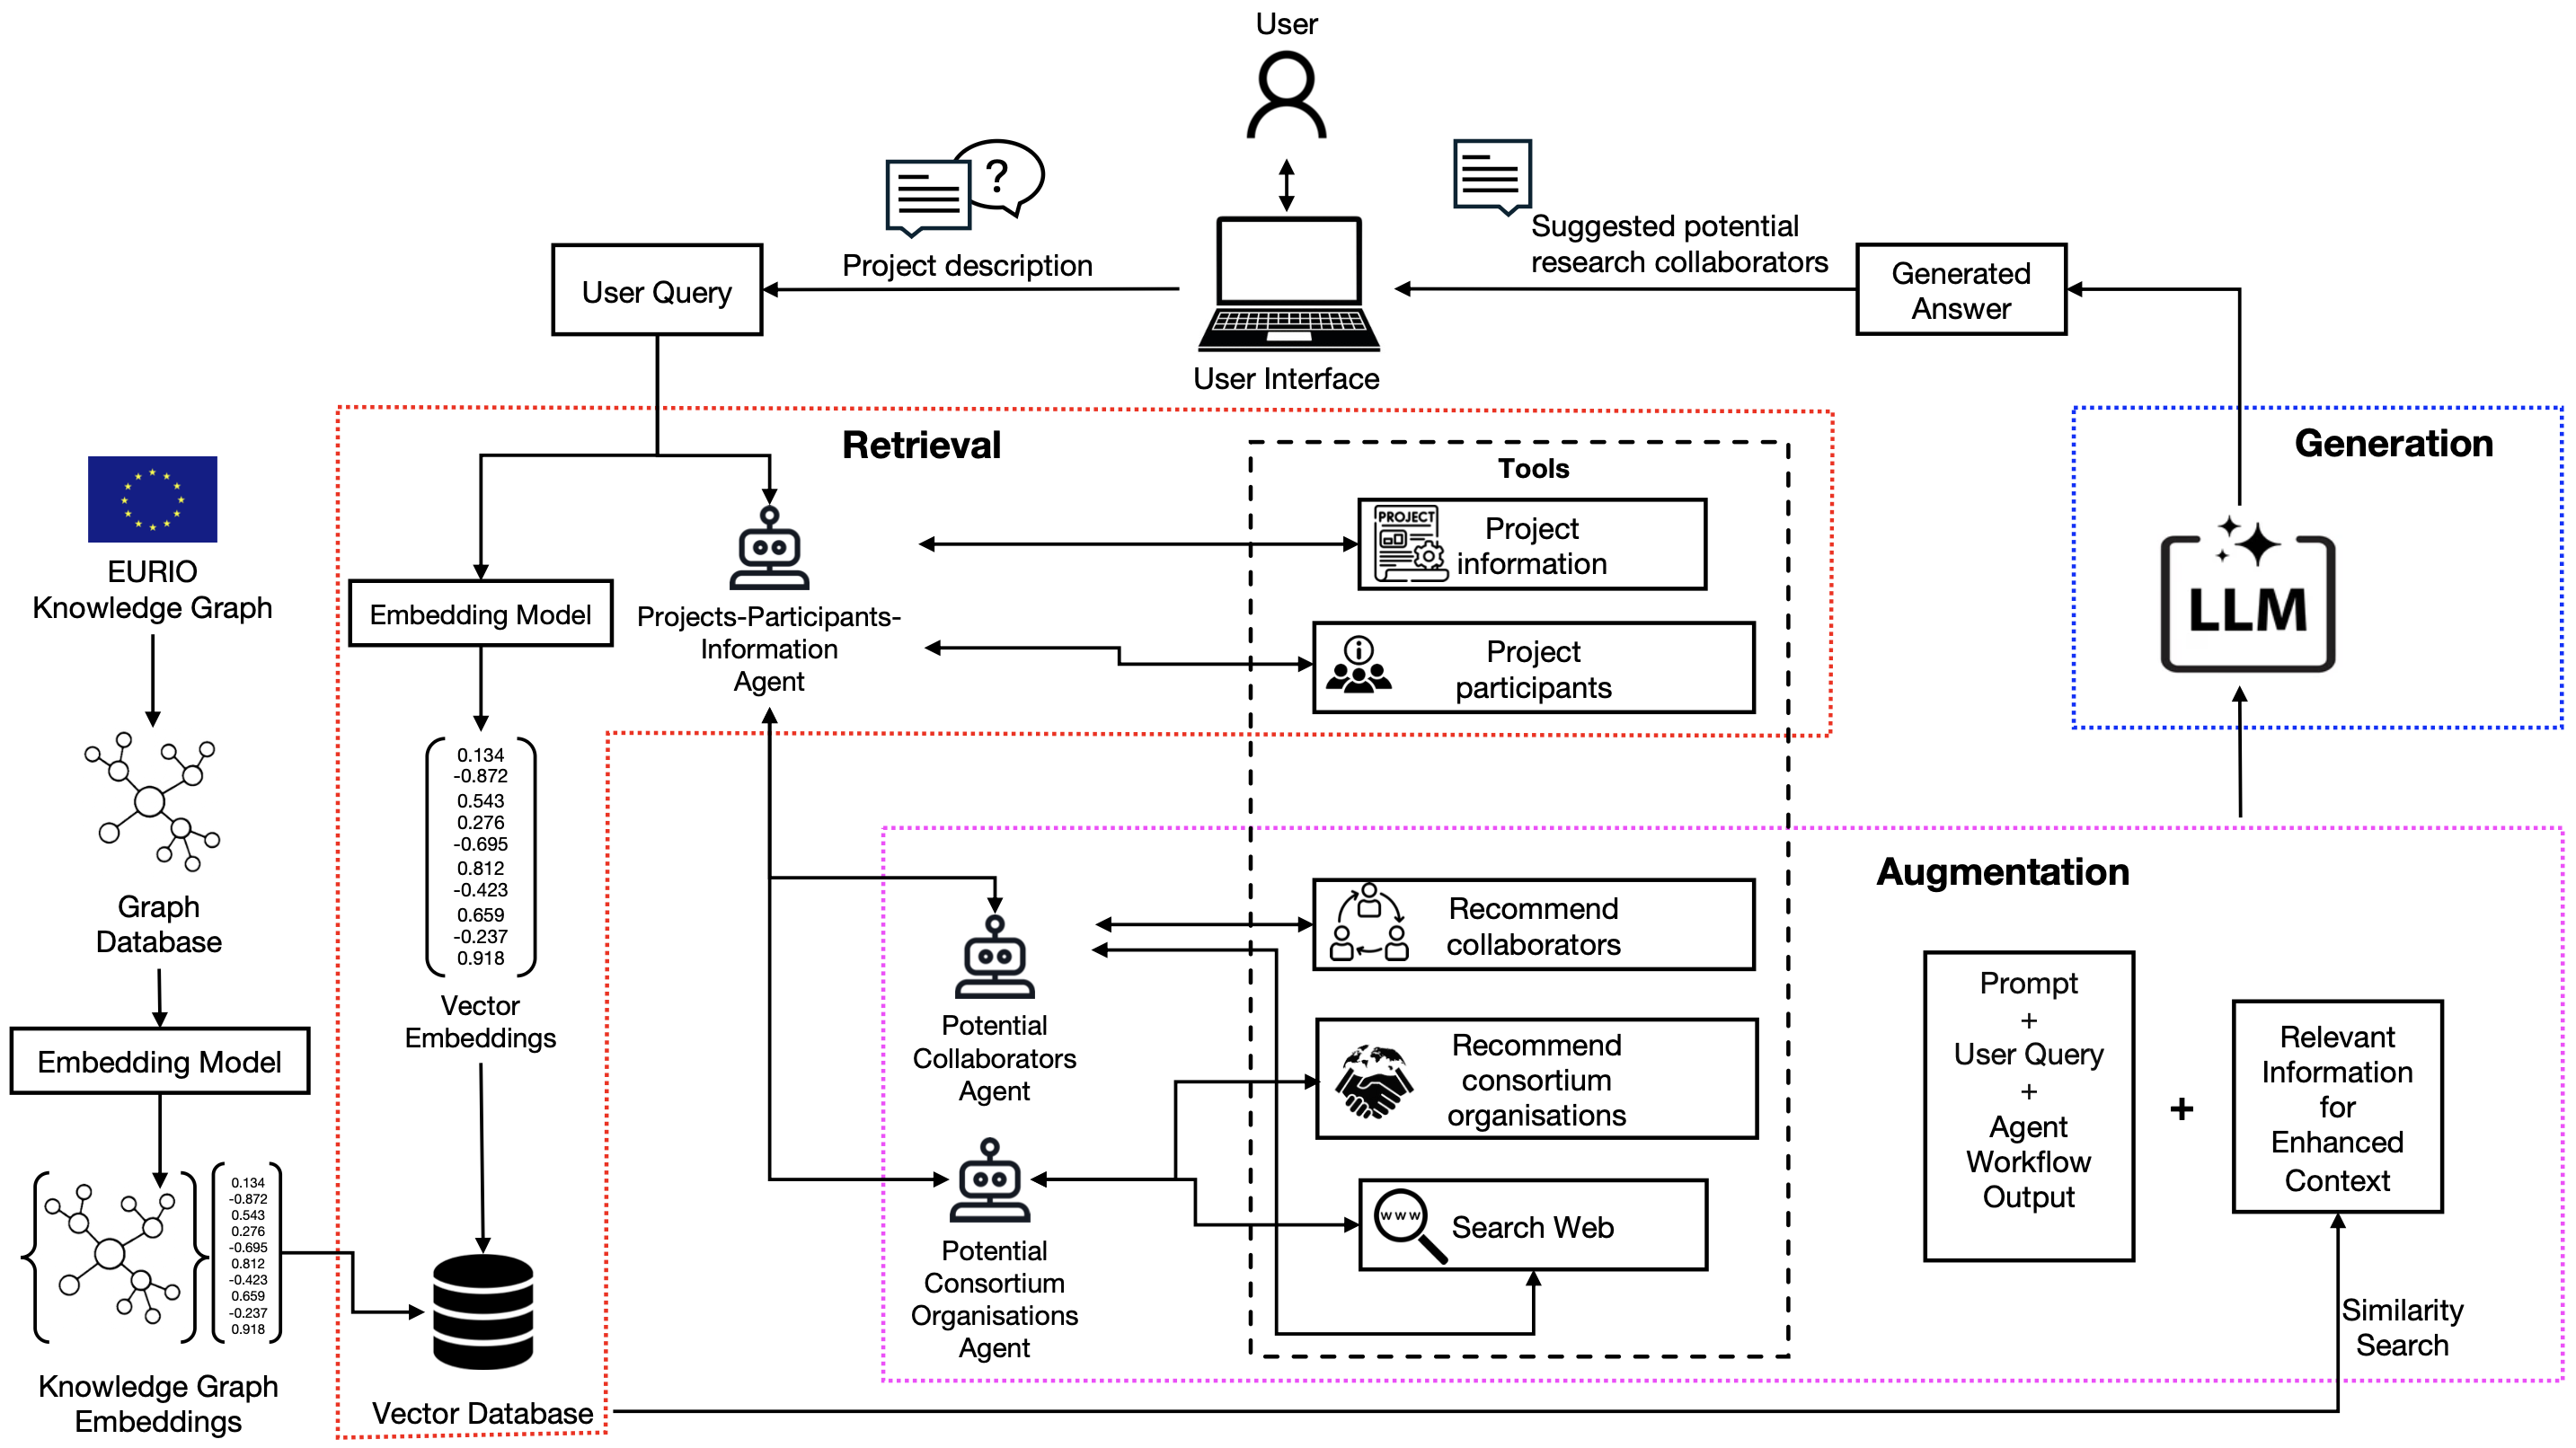
\includegraphics[width=\textwidth]{../img/architecture/proposed-system-graphRAG.png}
        %\caption{Artifact Architecture}
    \end{figure}

\end{frame}
%
\section{Technology stack}
\begin{frame}{Technology Stack}
    \begin{figure}
        \centering
        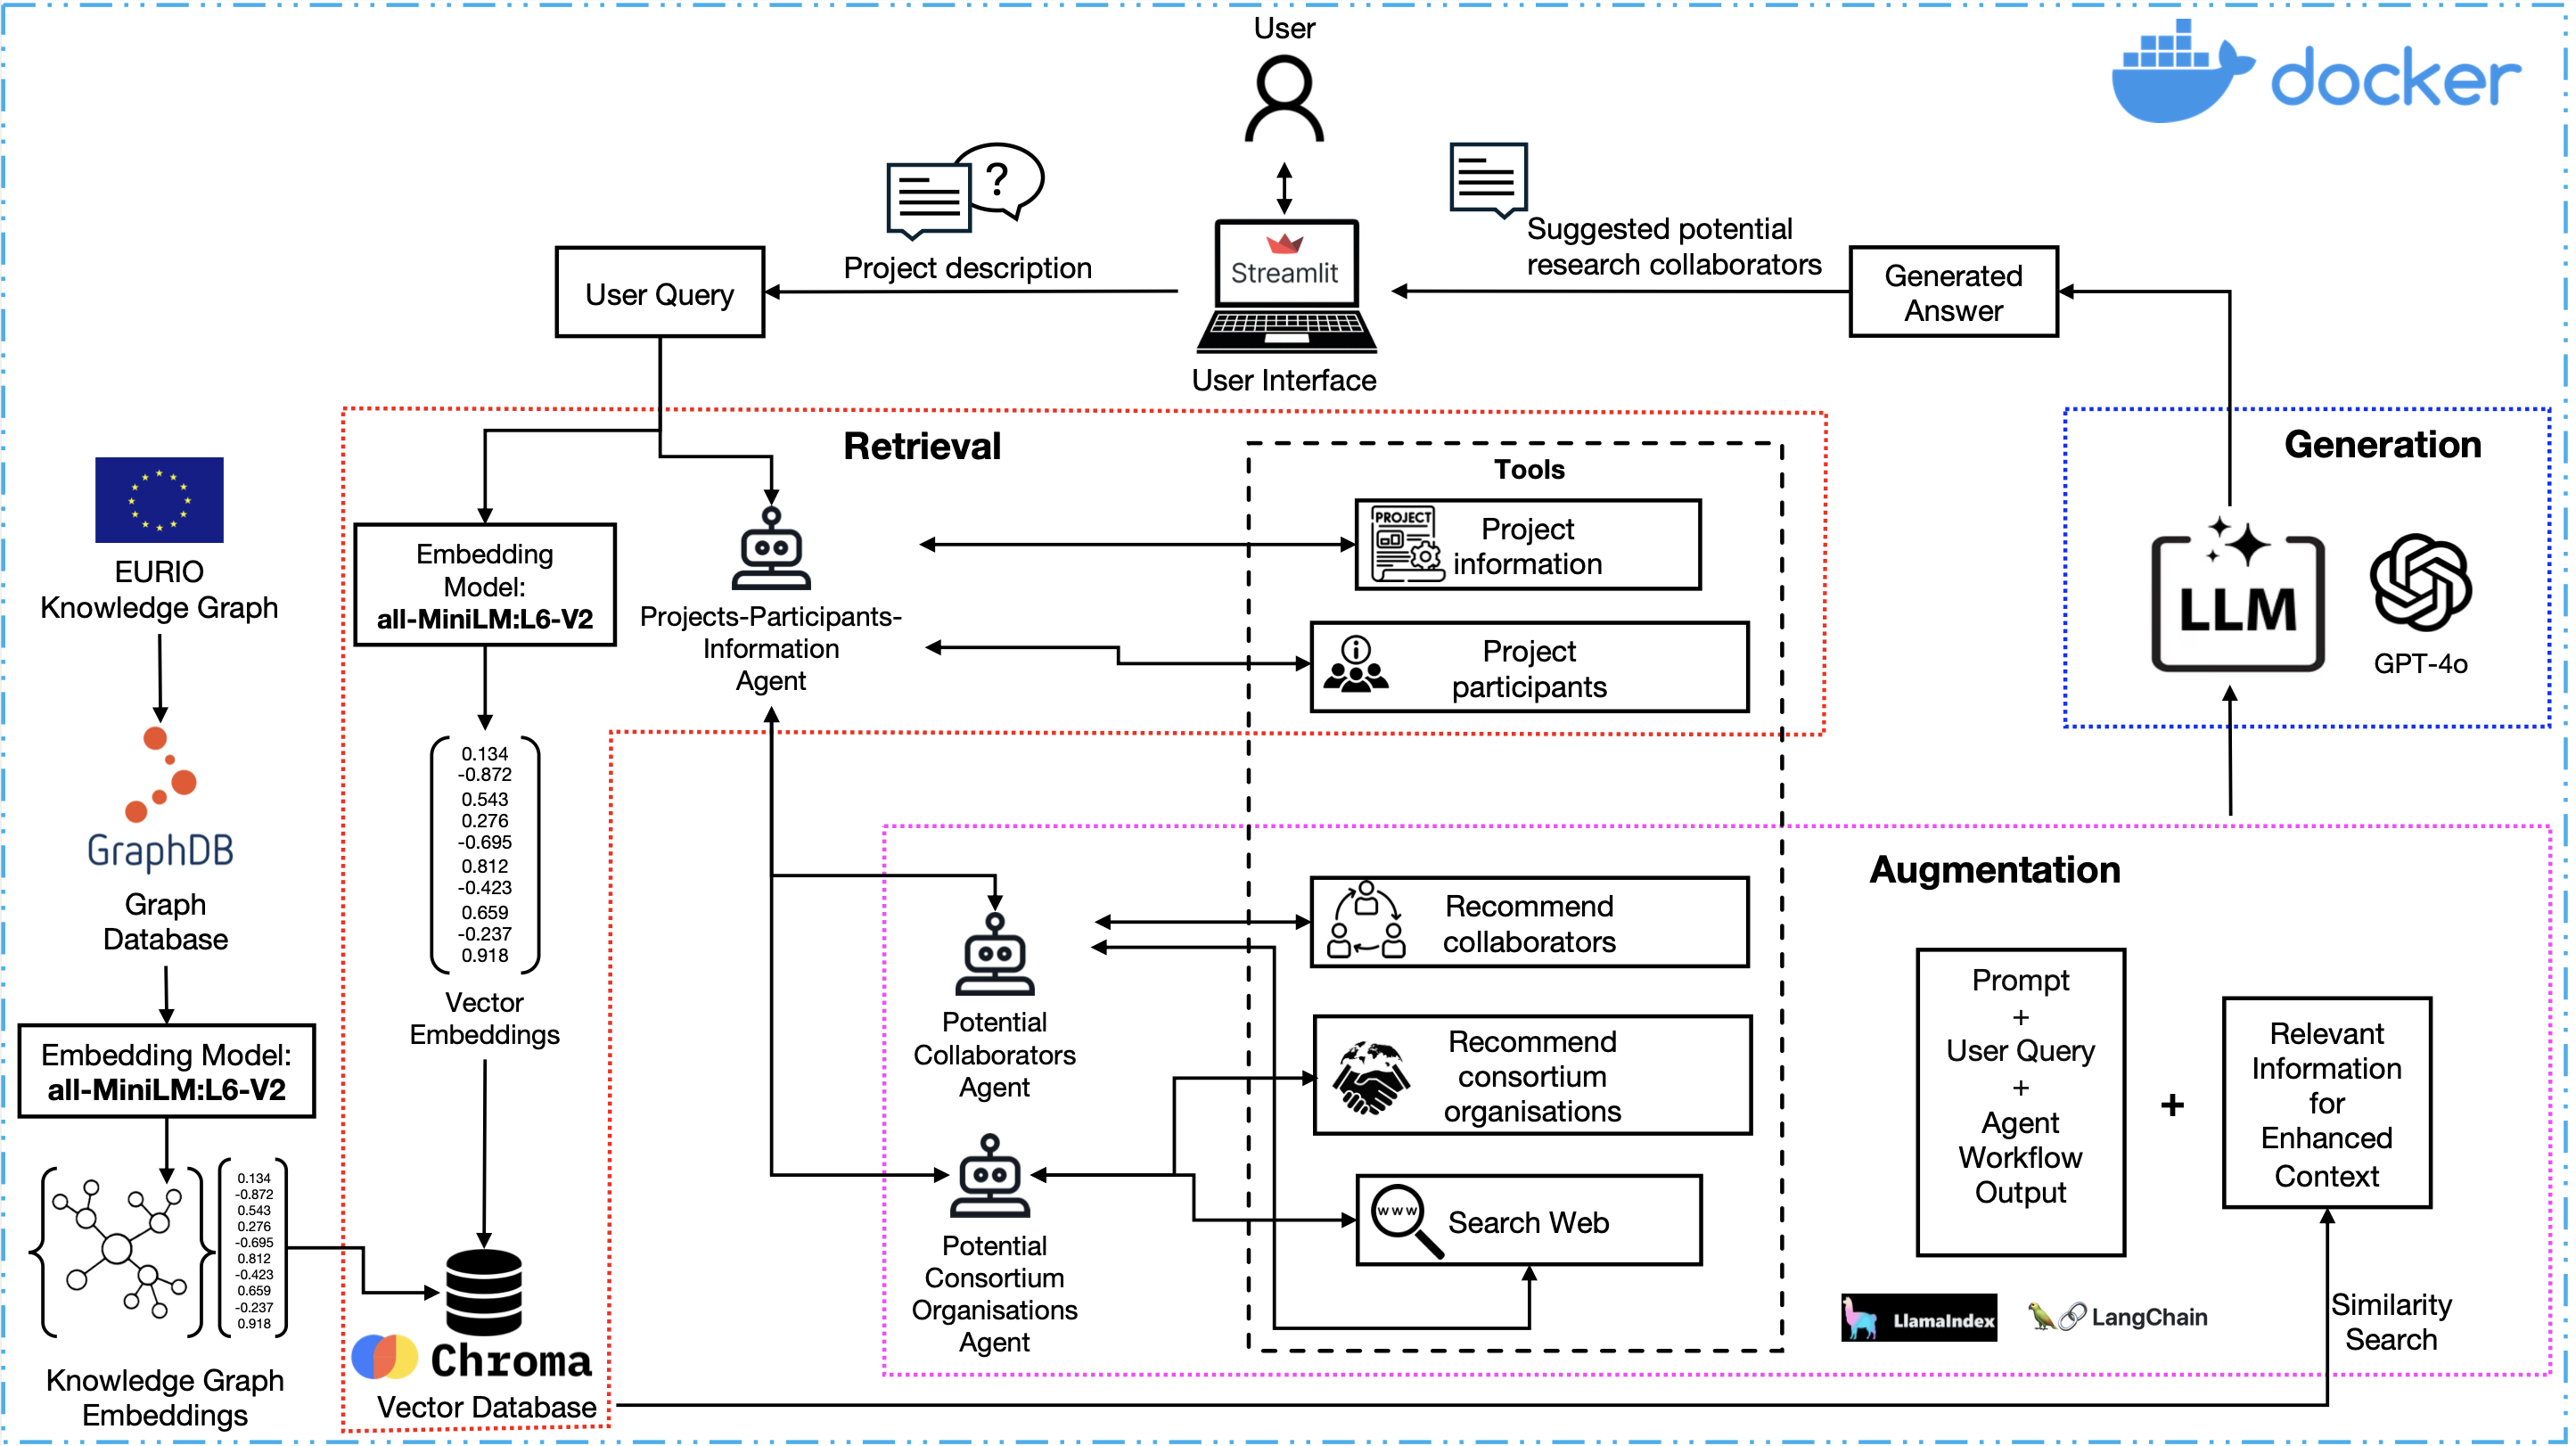
\includegraphics[width=\textwidth]{../img/implementation/proposed-system-graphRAG-technologies.png}
        %\caption{Artifact Architecture}
    \end{figure}
\end{frame}
%
\section{Evaluation}
\begin{tframe}{Evaluation}
\textbf{Goal:} Evaluate the performance of the Agentic Graph \gls{rag} pipeline for collaborator and consortia recommendations.

\vspace{0.5em}

    \textbf{Evaluation Framework:} \gls{ragas}~\cite{ragas2024}
    \begin{itemize}
    \item Assesses both \textbf{retriever} and \textbf{generator} components
    \item Quantitative evaluation using automatic \gls{llm}-based metrics
    \end{itemize}

    \vspace{0.5em}

    \textbf{Retriever Metrics:}
    \begin{itemize}
    \item \textbf{\gls{cp}}: relevant chunks at top ranks
    \item \textbf{\gls{cr}}: how well context supports the answer
    \item \textbf{\gls{cer}}: entity overlap between ground truth and retrieved context
    \end{itemize}
\end{tframe}
%
\begin{tframe}{Evaluation}
\textbf{Generator Metrics:}
    \begin{itemize}
    \item \textbf{Faithfulness}: factual consistency with context
    \item \textbf{\gls{ar}}: alignment with user prompt
    \item \textbf{\gls{ss}}: similarity to ground truth answer
    \item \textbf{\gls{ac}}: combined semantic and factual accuracy
    \end{itemize}

    \textbf{Evaluation Datasets:}
    \begin{itemize}
    \item Two manually annotated sets:
        \begin{itemize}
            \item potential collaborator recommendations
            \item potential consortia recommendations
        \end{itemize}
    \item 21 queries each, derived from real EU project descriptions
    \end{itemize}
\end{tframe}
%
\begin{frame}{Evaluation: Query Example}

%\vspace{-.2cm}

\scriptsize
\texttt{Project Description:}

\texttt{`The project aims to advance Artificial Intelligence (AI) for Connected, Cooperative, and Automated Mobility (CCAM) by enhancing situational awareness, predictive decision-making, and safety in time-critical scenarios.
The initiative will develop AI-driven solutions that integrate seamlessly with active safety systems while ensuring trustworthy, explainable, and human-centric AI to increase public acceptance and usability.
The project will focus on predictive system state awareness, moving beyond current reactive and adaptive AI approaches to anticipatory AI-driven automation.}

\ldots

\texttt{Project Objectives:}

\texttt{• OBJ1: Develop AI-based situational awareness, prediction, and decision-making models to improve safety-critical CCAM applications.}

\texttt{• OBJ2: Enhance AI training and validation methodologies by leveraging real and synthetic traffic event datasets, ensuring unbiased and ethical AI development.}

\ldots

\texttt{Which organisations could be potential collaborators to form a consortium for the specified project description and objectives?}
\end{frame}
%
\begin{tframe}{Results}
Values closer to 1 denote better performance; near 0 indicate worse.

\begin{center}
    \textbf{Collaborators Recommendation Evaluation Results}
    \begin{table}
        \centering
        \begin{tabularx}{\textwidth}{|X|c|c|c|c|c|c|}
          \hline
          \textbf{Faithfulness} & \textbf{\gls{ar}} & \textbf{\gls{cp}} & \textbf{\gls{cr}} & \textbf{\gls{cer}} & \textbf{\gls{ss}} & \textbf{\gls{ac}} \\
        \hline
        0.140 & 0.249 & 0.630 & 0.464 & 0.299 & 0.791 & 0.753 \\
        \hline
    \end{tabularx}
    %\caption{Collaborators Recommendation Evaluation Results}
    %\label{table:collaborators-recommendation-evaluation-results}
    \end{table}
\end{center}
\vspace{.2cm}
\begin{center}
    \textbf{Consortium Organisations Recommendation Evaluation Results}
    \begin{table}
        \centering
        \begin{tabularx}{\textwidth}{|X|c|c|c|c|c|c|}
        \hline
        \textbf{Faithfulness} & \textbf{\gls{ar}} & \textbf{\gls{cp}} & \textbf{\gls{cr}} & \textbf{\gls{cer}} & \textbf{\gls{ss}} & \textbf{\gls{ac}} \\
        \hline
        0.436 & 0.525 & 0.733 & 0.604 & 0.457 & 0.783 & 0.736 \\
        \hline
    \end{tabularx}
    %\caption{Consortium Organisations Recommendation Evaluation Results}
    %\label{table:collaborators-recommendation-evaluation-results}
    \end{table}
\end{center}

{
    \scriptsize
    \begin{columns}
        \begin{column}{0.48\textwidth}
    \begin{itemize}
        \item \textbf{\gls{ar}}: \acrlong{ar}
        \item \textbf{\gls{cp}}: \acrlong{cp}
        \item \textbf{\gls{cr}}: \acrlong{cr}
    \end{itemize}
\end{column}
\begin{column}{0.48\textwidth}
  \begin{itemize}
    \item \textbf{\gls{cer}}: \acrlong{cer}
        \item \textbf{\gls{ss}}: \acrlong{ss}
        \item \textbf{\gls{ac}}: \acrlong{ac}
    \end{itemize}
\end{column}
\end{columns}
}

\end{tframe}
%
\section{Conclusion}
\begin{tframe}{Contribution}

    \textbf{Main Research Question}:
    \begin{center}
        \textit{How can a \gls{kg} and \gls{llm}-based approach enhance the process of suggesting collaborators for research projects?}
    \end{center}

    \textbf{Research contributions}:
        \begin{itemize}
            \item Investigated the limitations of existing approaches for suggesting collaborators.
            \item Proposed an approach that leverages \glspl{kg} and \glspl{llm} to enhance the research collaboration process.
        \end{itemize}

        \vspace{0.2cm}

    \textbf{Application contributions}:
        \begin{itemize}
            \item Designed and developed a user-friendly system for recommending research collaborators using real-world data
            \item Demonstrated the system's ability to retrieve and explain relevant collaborator recommendations using semantic enrichment
        \end{itemize}
\end{tframe}
%
\begin{tframe}{Future Directions}
    \begin{itemize}
        \item \textbf{Automatic updating of the \gls{kg}} (including information about Horizon Europe projects) to keep up with emerging research topics and thus keep the proposed approach relevant over time
        \item The \textbf{integration of academic \glspl{kg}} could be a useful resource to enrich the \gls{eurio} knowledge base and thus add context regarding the recommendation of papers and researchers.
        \item The construction of \textbf{more detailed evaluation datasets} provided by experts could be future work that could help improve the artifact evaluation
    \end{itemize}
\end{tframe}
%
\begin{tframe}{Conclusion}
    \textbf{Agentic Graph \gls{rag}} was introduced to deliver contextual and explainable recommendations for research collaborators by combining \textbf{\glspl{kg}} and \textbf{\glspl{llm}}.
    
    \vspace{0.5em}
    \textbf{Evaluation Highlights:}
    \begin{itemize}
      \item High-quality and contextual reasoning, reduced hallucinations
      \item Areas needing improvement: \textit{consistency} and \textit{context retrieval}
    \end{itemize}
    
    %\vspace{0.5em}
    \begin{columns}
      \begin{column}{0.52\textwidth}
        \begin{itemize}
          {\scriptsize
          \item This thesis work has been submitted to the \textbf{Society 5.0 conference}%\footnote{\url{https://www.conference-society5.org}}
          \item A journal version is in preparation for submission to the \textbf{Semantic-Web Journal}%\footnote{\url{https://www.semantic-web-journal.net/blog/special-issue-large-language-models-generative-ai-and-knowledge-graphs}}
          }
        \end{itemize}

        %\vspace{0.2cm}

      \end{column}
      \begin{column}{0.4\textwidth}
        %\vspace{-.5cm}
        \begin{figure}[htbp]
          \centering
          \rotatebox{-5}{\fbox{
\includegraphics[width=.75\textwidth]{../img/conclusion/society-paper.png}}}
      \end{figure}
      \end{column}
  \end{columns}
\end{tframe}
%
\begin{frame}{The End}
    \vspace{-.15cm}

    \begin{figure}[htbp]
        \centering
        
\includegraphics[width=\textwidth]{../img/thankyou-final.png}
    \end{figure}
    %\centering
    %\huge \textbf{Thank you for your attention!}
\end{frame}
\section*{References}
{
\setbeamertemplate{footline}{} % Disable footer just for this frame
\begin{frame}[allowframebreaks,noframenumbering]{References}
    %\nocite{*}
    \printbibliography
\end{frame}
}
\end{document}